\documentclass{article}

\usepackage[utf8]{inputenc}
\usepackage{graphicx} % Comandos para manejar imágenes
\graphicspath{ {./images/} } % Carpeta de imágenes

\setlength{\parskip}{2mm} % Espaciado

\usepackage[utf8]{inputenc}
\usepackage{geometry}
    \geometry{left=3cm,right=2cm,top=2cm,bottom=2cm}
%
%\usepackage[spanish]{babel}
%
\usepackage[fixlanguage]{babelbib}
    \bibliographystyle{babunsrt}
%

\usepackage{floatrow}
\floatsetup[table]{style=plaintop}

\usepackage{url}

\usepackage[top=2cm, bottom=2.5cm, right=3 cm, left=3 cm]{geometry} % margenes

\usepackage{parskip} % Sangria

\title{Seminar two: Wisdom of the flock, a brief comment on the presentation of Doctor Sebastián Cea}
\author{Cristóbal Galleguillos Ketterer$^{1}$\\
\small{$^{1}$Industrial PhD Program}\\
\small{Pontificia Universidad Católica de Valparaíso}\\
\small{cristobal.galleguillos@pucv.cl}
}
\date{\small{\today}}

\begin{document}

\maketitle

\section{Introducción}

This work presents a brief summary of the presentation by doctor Sebastián Cea called \textit {Common Beliefs and Welfare: Opposite beliefs sharing a similar results}\cite{art1:articulo1}, in this work we propose to we approximated to the study of the relationship between equity and efficiency for a specific market (welfare and goods).

The work of doctor Cea starts from an investigation of theoretical mathematics taken to the field of applied theory \cite{art2:articulo}\cite{art3:articulo}\cite{art4:articulo}, during the development of the work, the data of the World Values Survey (WVS) was seen. the survey is long-standing, which allows having an adequate time series and is based on two premises on interpersonal trust:

\begin{itemize}
   \item People trust most people.
   \item People take care with other people
\end{itemize}

\subsection{Scope}

In this work, the formulations mathematical of models and their demonstrations are deliberately excluded. For the interested reader these are indicated in the bibliography-

\section{Literature review}

The doctor Cea is an investigator in the areas of economics and mathematics, to start to the revision of your investigations is possible to identify your principal interests in the following figure

\begin{figure}[H]

\includegraphics[scale=0.5]{Images/Nube de palabras.jpg}
\centering
\caption{Main words}
\label{etiqueta}
\end{figure}

In the specific area of investigation of doctor Cea, from ScienceDirect data, it is possible visualized an increment of this type of investigation, proof of the importance of the articulation between economics, mathematics, and psychological issues (see Keywords \cite{art1:articulo1}) . The tendency is shown bellow.

\begin{figure}[H]
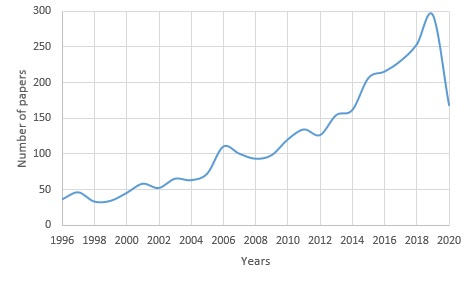
\includegraphics[scale=0.5]{Images/Tendencia.jpg}
\centering
\caption{Main words}
\label{etiqueta}
\end{figure}

\section{Framework}

To explain the framework of the work presented by doctor Cea, is possible to inquire in the mathematical theory that sustain the model, but this aspect is excluded explicitly in the scope. The reader will be able to find in the bibliography abundant information about this theme.

We understand the problem as a phenomenon sociological, and in this terms, we will try to tackle in in two interesting texts, what the complex relationship between welfare and goods.

According to doctor Peña \cite{lib1:libro} this reflection define your place in the wold and this provides a set of competencies to lives in the world (lives is works, eat, enjoy, welfare and goods in definitive). 

The author indicated a Bourdieu and Marx like philosophers what thinking what the individuals makes your own history, but not know the history do they do.

Is this not a theoretical paradigm that Doctor Cea presents in his study about the relationship between well-being and goods?

In your exposition, the doctor Cea speak about a mental experiment, One individual "one" forget your wallet in a public place, another individual (individual "two") have two options, cooperation or no cooperation: ¿What history decide to write the individual "two"? ¿He is conscious of the "awards" of the games? ¿The simple (or complex) psychology of this decision is sufficient for the individual "two" take the choice what maximized the welfare?.

En another case (and other individuals), the doctor Engel \cite{web1:web} speak of the "Overconfidence bias" in the case of the final decision to take the wallet, for the individual "two", and he is discovered and taken to prison, the strategies of the gamer's depend on en great measure in the quality of information, the precision of this an the opportunity. Also es important to assume strategies conservatives and be careful.

The analysis of the doctor Engel is in a base an particular scenario (different a mentioned for the doctor Cea) but, in this cited articles of doctor Peña and doctor Engel, we situated in a camp situated between the economics and the psychology.

Its is a generic framework, yes, but we speak about human behavior  against the economic stimulus

\section{Author's Contribution}

The work analyzed in this inform, its an extension of the work \cite{art5:articulo}, in this work the author proposal mathematical model when the "agents choose consumption—but they also choose which firms to join, which roles to occupy in those firms, and which actions to take in those roles". 

The strategy proposal include what the  "Agents interact anonymously with the (large) market, but strategically within the (small) firms they join. The model accommodates moral hazard, adverse selection, signaling, and insurance. Equilibrium may be Pareto ranked"

In this work is presented a game name moral hazard what consider a world with two goods and a single  kind of productive activity. This game Production requires the participation of two agents.

The output is observable and contractible but effort is not, so each member provides half the input and receives half the output.

The game is described mathematically and it give the equilibrium and strategies dominants.

The extensions "provide foundations for the discussion of how beliefs and welfare relate", for this it's used a general equilibrium setup in which anonymous interactions take place. 

The economy is parametric for an extension of a game presented in \cite{art5:articulo} for a set of propositions whit different combinations between benefits and good.

This models presents an aleatory process, and asymmetric relationships, similar a traditional game like the prisoner games.

Whit this model the authors exploration of common beliefs using the data for the WVS. This analysis "suggests that the payoffs of the interaction induce strategic behavior such that in most cases, the proportion of agents participating in the productive interaction, efficiency, and welfare are directly related to optimistic or virtuous beliefs"

Inside the work, an interesting question is explored, like as the port tramps, what its the causes of a same country existing different levels of trust or welfare or when the trust o welfare of one country its comparable whit other countries

\section{Additional comments}

\subsection{Point of view: Psychology of the organization }

In several countries, furthermore of the person concept, 
exist the definition of a juridical person, what give a corporation the majority of the right and obligations of a natural person.

For the corporations case, the net profit is quantified for the utility at the final of a period, but, at the last times, the juridic persons are evaluated by the society, starting off what we could call the "the neighbor's behavior", for example (only Chilean cases):

\begin{itemize}
    \item The collusion of the paper hygienic in Chile.
    \item Greatest port and mineral projects.
    \item Charitable roles (like as Teleton)
\end{itemize}

Its possible to evaluate impacts on the prices or the offers of the consumers and the surplus of the society versus this conducts of the corporations and the sanctions (or awards like taxes exceptions) of the regulator?

From the line of work of doctor Cea, we can speak of the psychology of the organization and the relation whit the confiance of the society and for addition the welfare of the consumers and producers in the classic economic equilibrium.

It is a good model, o good start, the model a "carrot, and stick" strategies of the game theory?

\subsection{Point of view: Political affairs}

In the work of doctor CEA, it study a proposition of the comportment of two agents interacting on a market, these choices are related whit the beliefs, efficiency, and welfare. 

Starting to the work of the doctor Cea, it's possible include, a regression analysis, and include estimators, that allows considering
the political/economical cycles like:

\begin{itemize}
    \item Approbations levels of the government.
    \item Economic growth.
    \item Schooling level.
\end{itemize}

\subsection{Point of view: Mental (impossible) social experiment}

To finish the work, we propose an imaginary experiment about the welfare and the political issues, in the image sown belly, we present a diagram a fictional word, whit to groups of control, the first is government by a traditional parliament representative of political forces, and more or less democratic.

The second group is governed by a random parliament, representative exactly of the composition (racial, political, sexual, religious) of the population.

Both groups are exposed to the same ambient conditions.

How to play the different groups?
How would the relative importance of welfare versus goods?
Is important the election capacity versus representative sensation?

And the main thing, is it possible to make a mathematical model for this?

\begin{figure}[H]
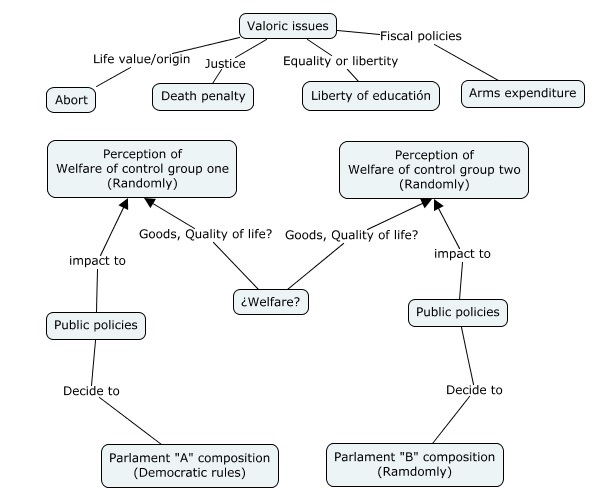
\includegraphics[scale=0.5]{Images/Experimento mental.jpg}
\centering
\caption{Main words}
\label{etiqueta}
\end{figure}





\nocite{*}
    \bibliography{src/ref}

\end{document}
